\section{Interface utilisateur}

Le site utilise Bootstrap pour déployer un thème responsive et robuste.
Dans un premier temps, les utilisateurs arrivent sur la page d'accueil (voir
\ref{fig:index}) sur laquelle le menu est présenté. Une barre de navigation
donne accès au livre d'or, à la page d'inscription et à la page de connexion.
Lorsqu'un client est connecté, l'accès au panier de course et au bouton de
déconnexion.

\begin{figure}[H]
	\centering
	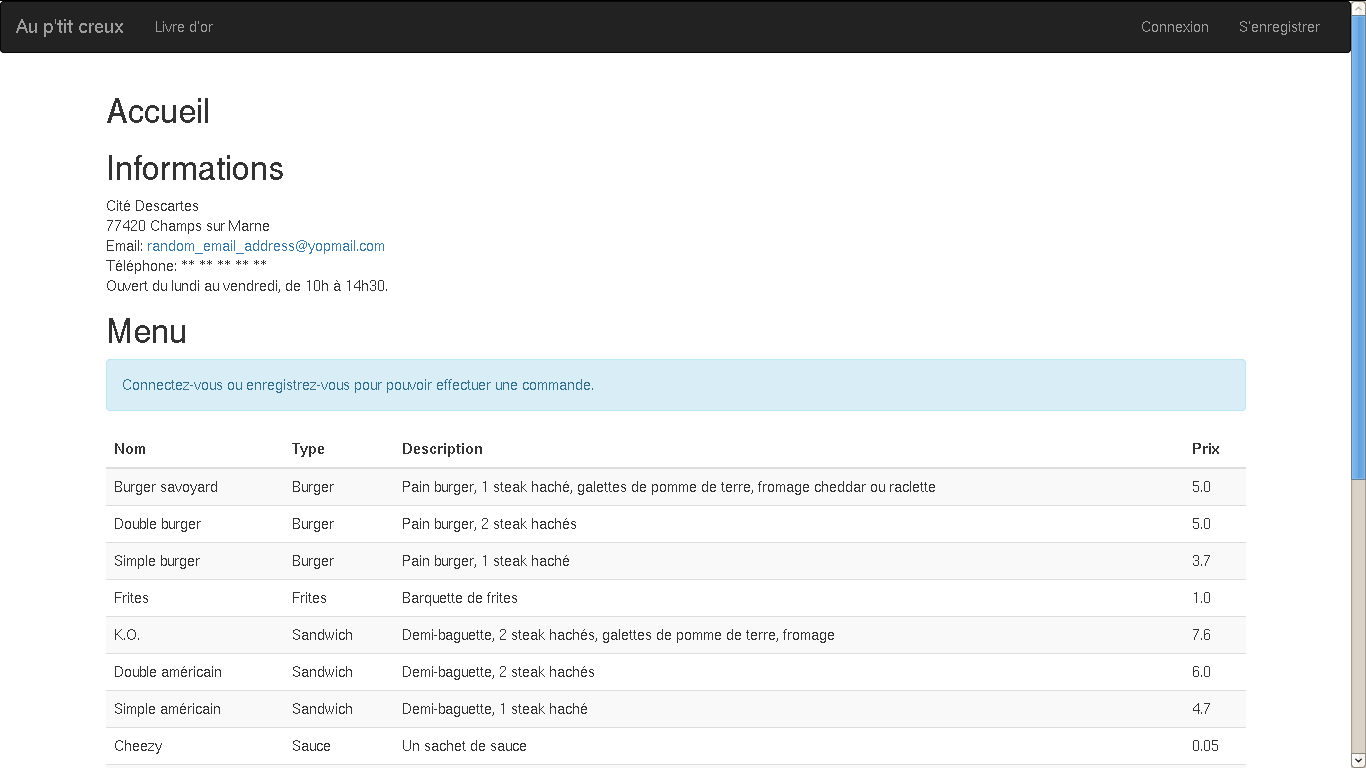
\includegraphics[width=0.8\textwidth]{res/index.png}
	\caption{Page d'accueil}
	\label{fig:index}
\end{figure}

Pour s'inscrire, l'utilisateur doit remplir un formulaire qui va peupler la
base de données. Le formulaire possède des validateurs d'expression pour
contrôler les données écrites par l'utilisateur.

\begin{figure}[H]
	\centering
	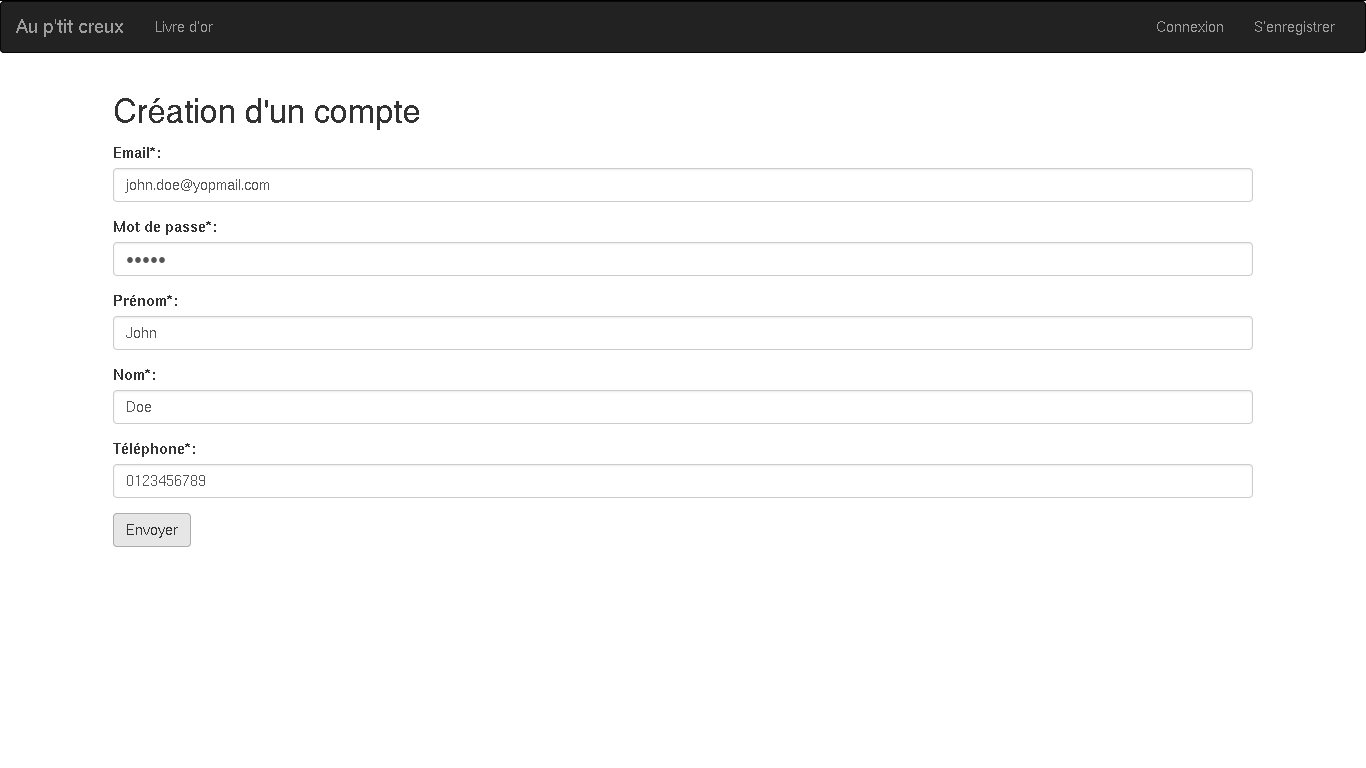
\includegraphics[width=0.8\textwidth]{res/formulaire_inscription.png}
	\caption{Formulaire d'inscription}
	\label{fig:signup}
\end{figure}

Après l'inscription ou une connexion, l'utilisateur est redirigé vers
l'index où il pourra sélectionner des produits à mettre dans le panier.

\begin{figure}[H]
	\centering
	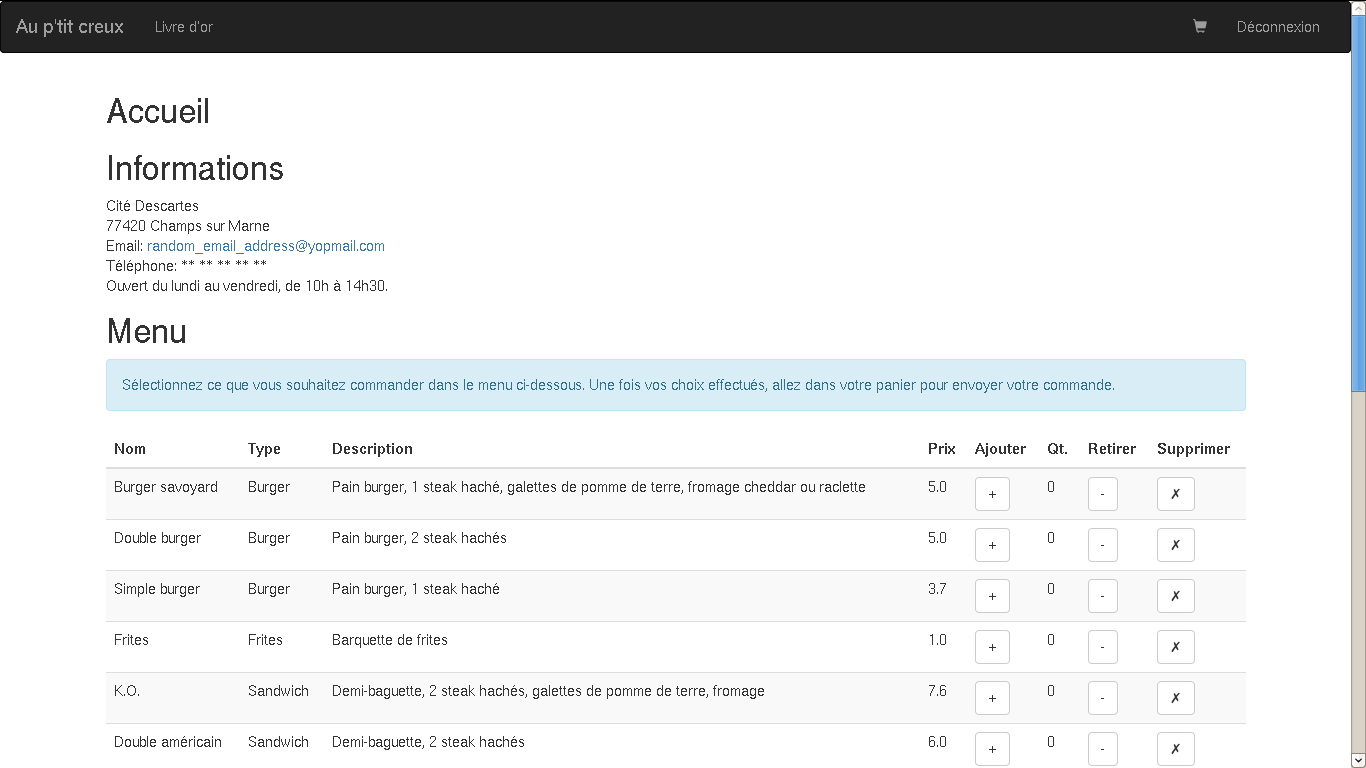
\includegraphics[width=0.8\textwidth]{res/afterConnexion.png}
	\caption{Index après connexion}
	\label{fig:logged}
\end{figure}

Sur la figure \ref{fig:logged}, des boutons pour ajouter, retirer des unités ou
supprimer des produits du panier sont affichés. Sur la page du panier, nous
retrouvons la liste des produits du panier et nous pouvons aussi retirer des
unités ou des produits. Enfin, on peut envoyer la commande au serveur qui
videra le panier.

\begin{figure}[H]
	\centering
	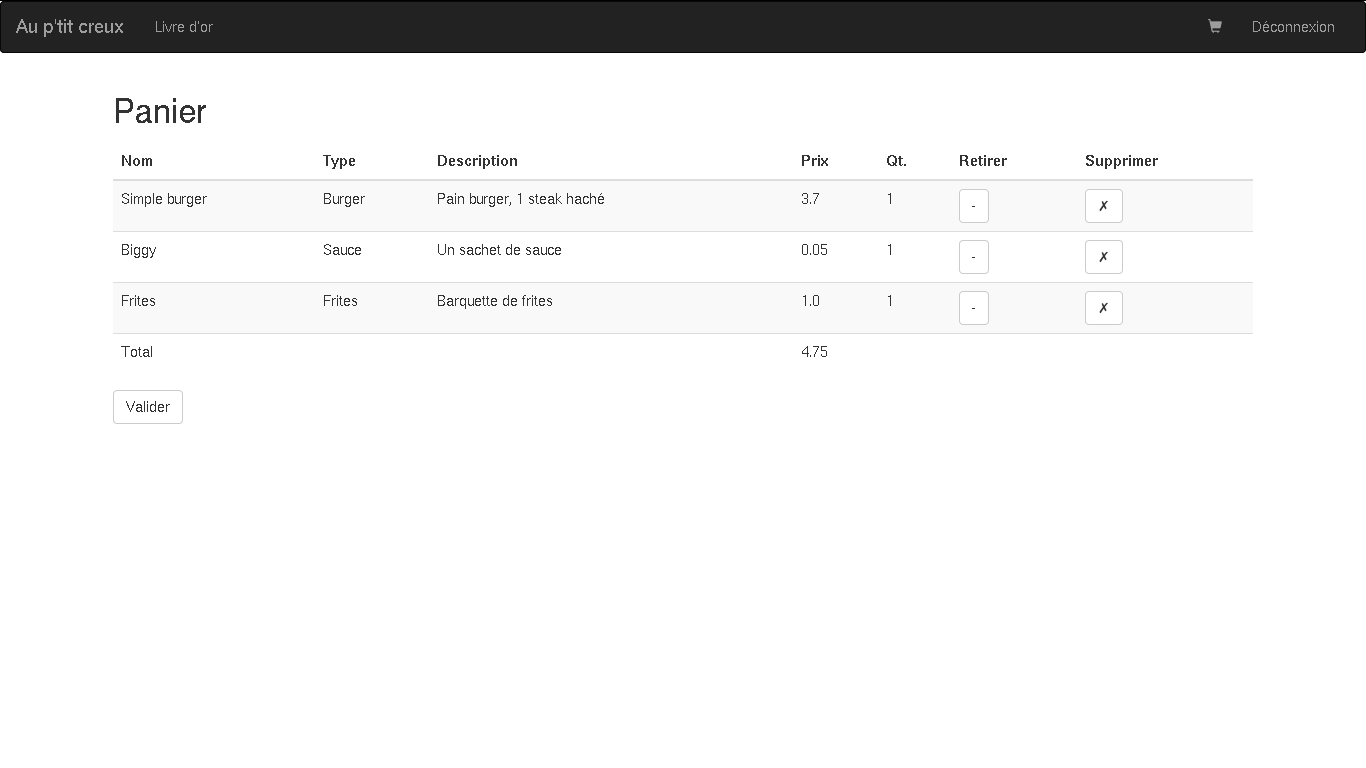
\includegraphics[width=0.8\textwidth]{res/panier.png}
	\caption{Aperçu du panier}
	\label{fig:cart}
\end{figure}

Le site possède également un livre d'or où on peut voir et ajouter des
commentaires sur le site.

\begin{figure}[H]
	\centering
	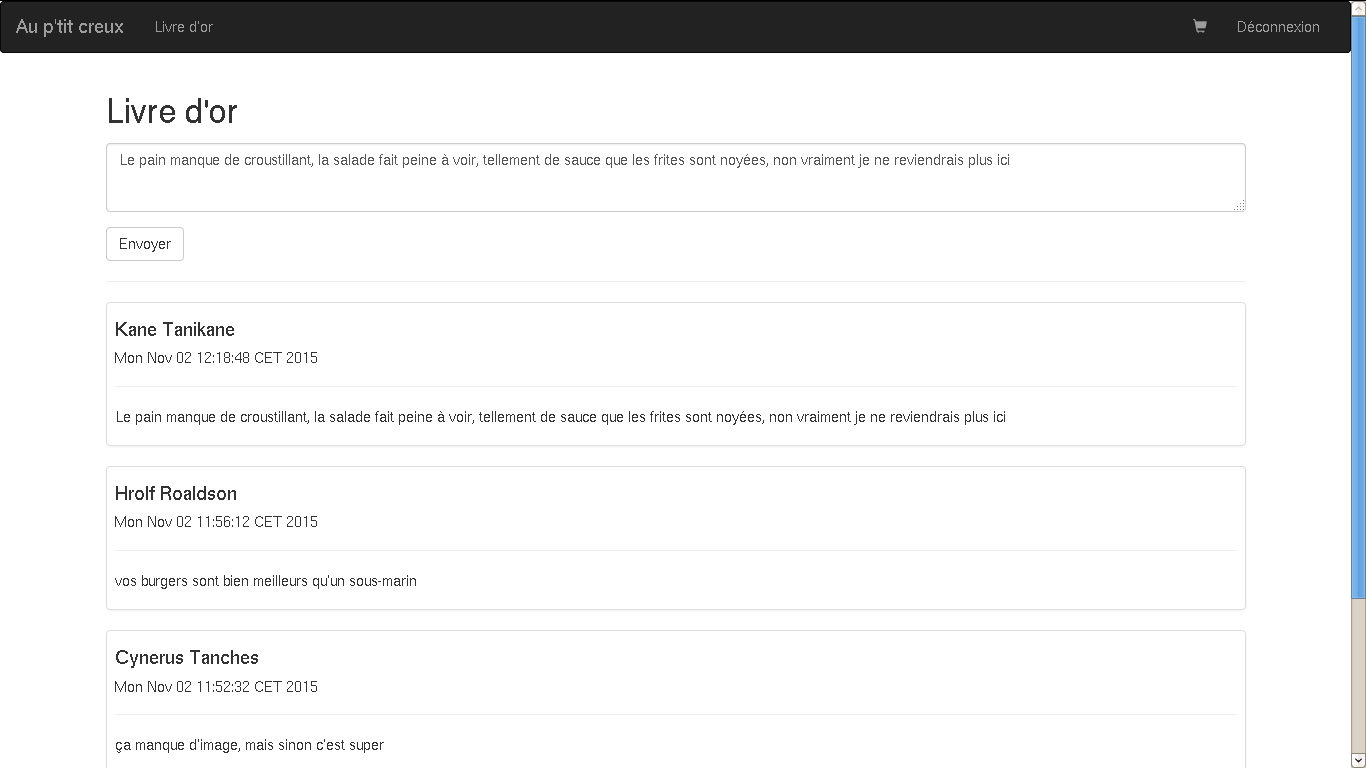
\includegraphics[width=0.8\textwidth]{res/livre_comment.png}
	\caption{Livre d'or}
	\label{fig:guestbook}
\end{figure}

Du côté administrateur, nous avons une interface de gestions des produits sur
laquelle on peut supprimer ou ajouter des produits.

\begin{figure}[H]
	\centering
	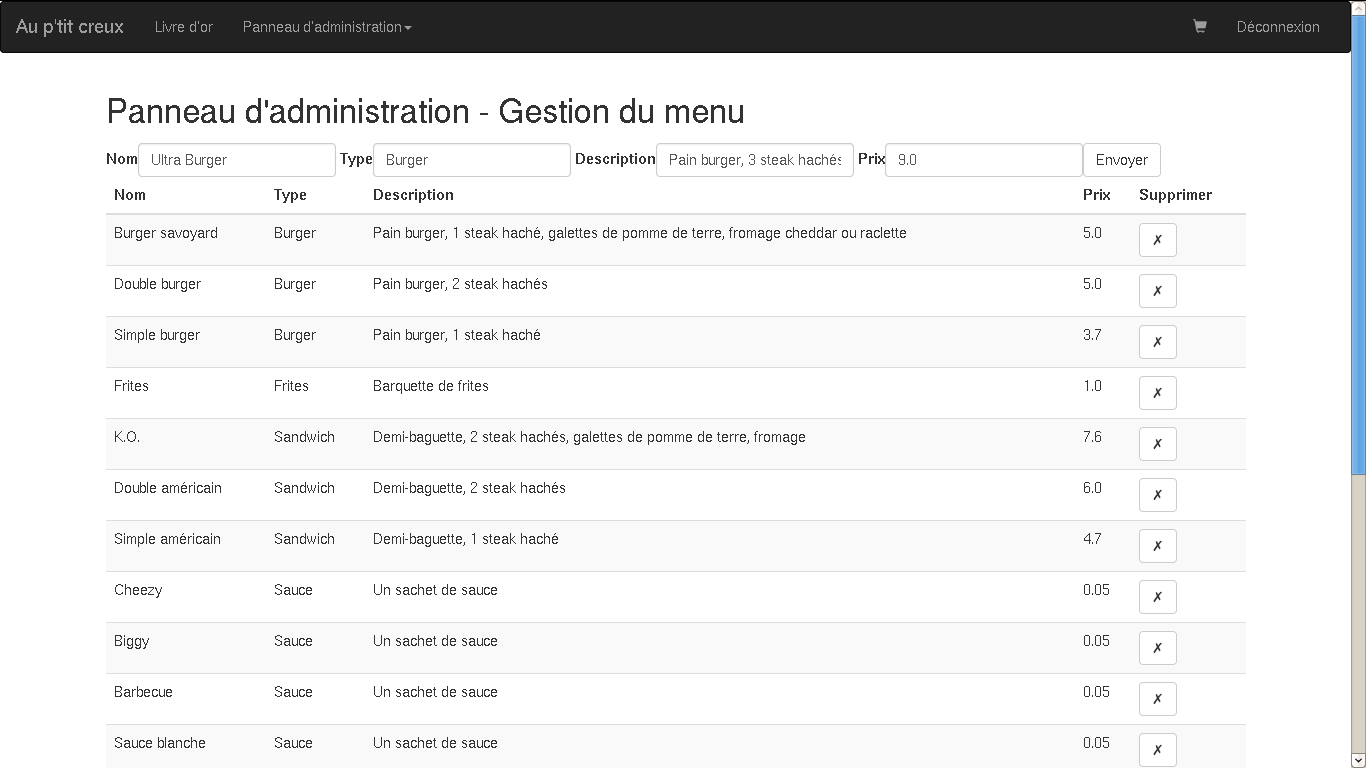
\includegraphics[width=0.4\textwidth]{res/ajout_burger.png} 
	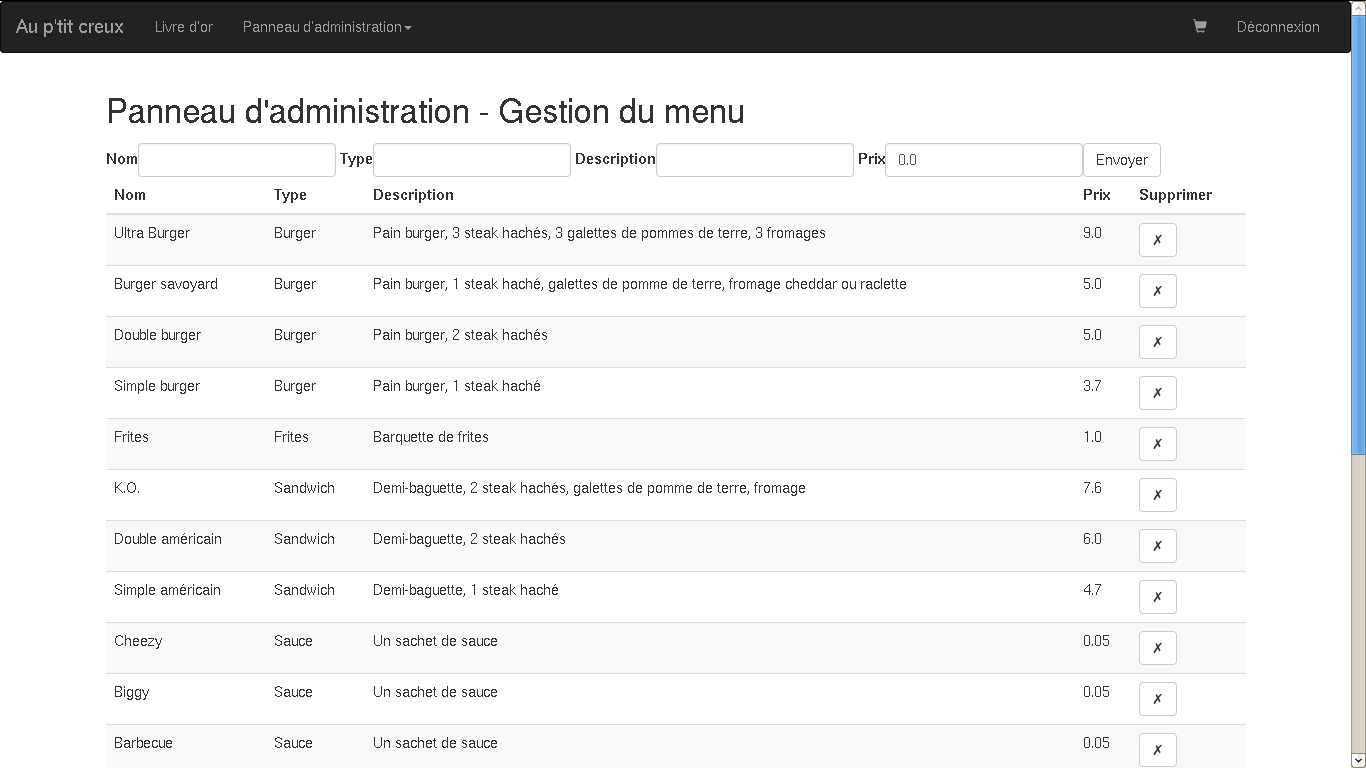
\includegraphics[width=0.4\textwidth]{res/ajout_burger2.png}
	\caption{Administration des produits}
	\label{fig:food_admin}
\end{figure}

Enfin, nous pouvons voir l'historique des commandes faites par les clients où
il est aussi possible de voir le contenu des paniers commandés.

\begin{figure}[H]
	\centering
	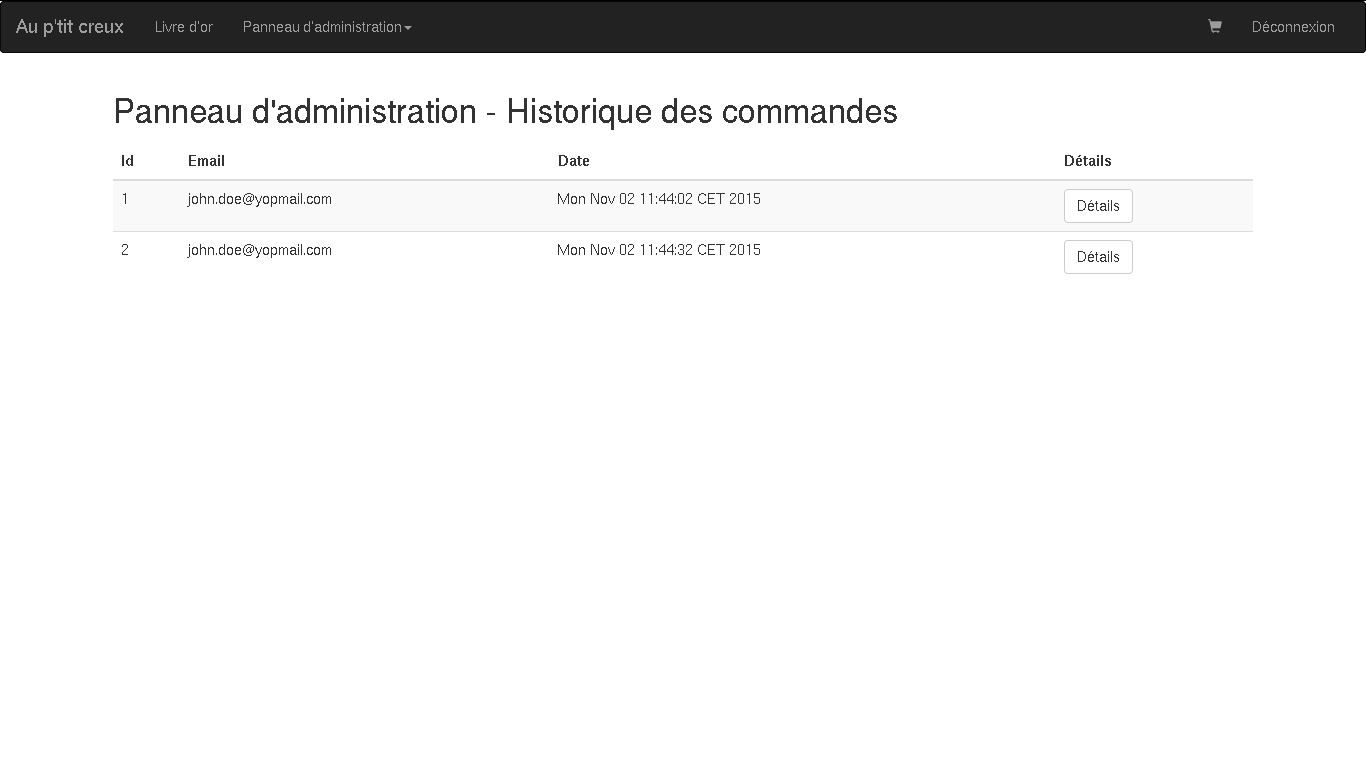
\includegraphics[width=0.4\textwidth]{res/admin_histo1.png} 
	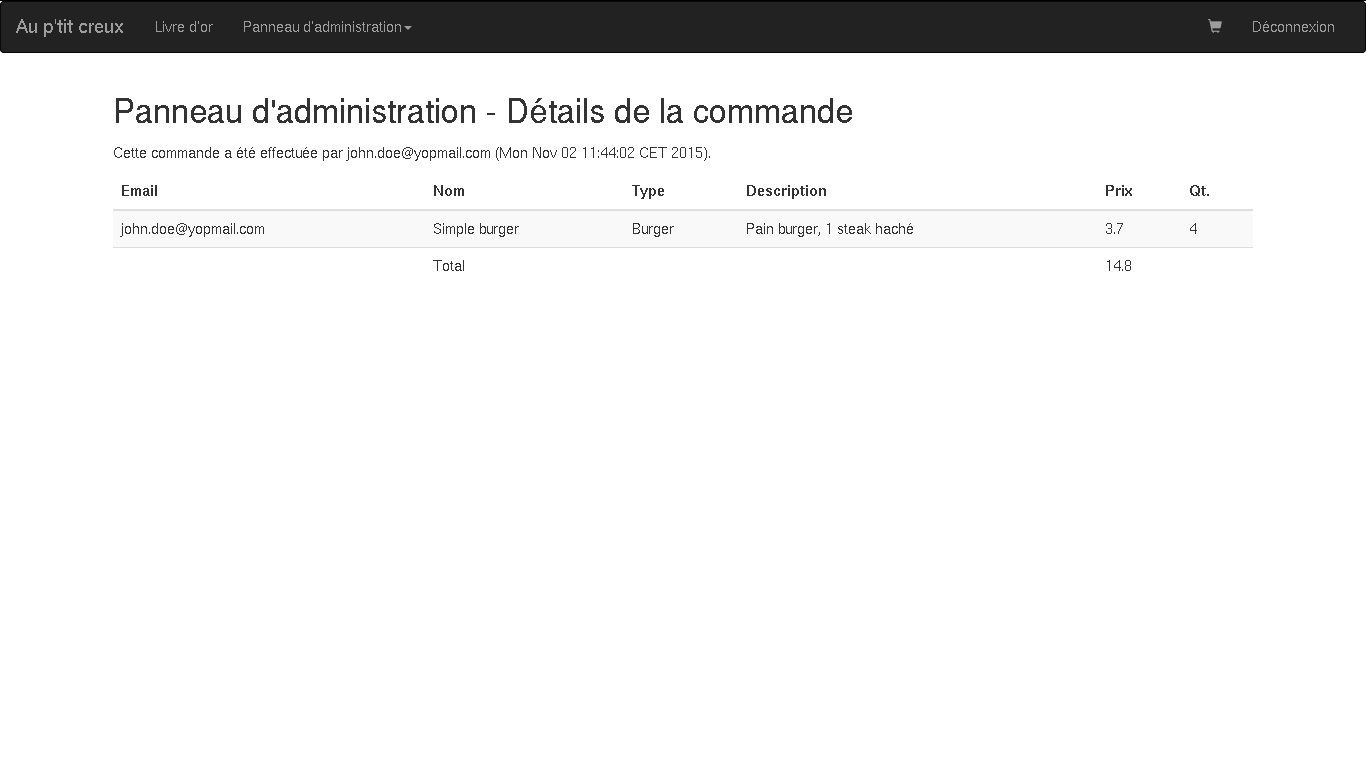
\includegraphics[width=0.4\textwidth]{res/admin_histo2.png}
	\caption{Administration des commandes}
	\label{fig:order_admin}
\end{figure}

